\chapter{Concorrenza}
\newpage

\section{Introduzione alla concorrenza}
\subsection{Modello concorrente}
Un sistema operativo consiste in un gran numero di attività che vengono eseguite più o meno contemporaneamente dal processore e dai
dispositivi presenti in un elaboratore.

Senza un modello adeguato, la coesistenza delle diverse attività sarebbe difficile da descrivere e realizzare.

Il modello che è stato realizzato a questo scopo prende il nome di
modello concorrente ed è basato sul concetto astratto di processo.

\paragraph{In questa serie di lucidi:} analizzeremo il problema della gestione di attività multiple da un punto di vista astratto.

Il modello concorrente rappresenta una rappresentazione astratta di
un S.O. multiprogrammato.

\paragraph{Negli altri moduli del corso:} vedremo i dettagli necessari per la gestione di processi in un S.O. reale.

In particolare, il problema dello scheduling, ovvero come un S.O.
seleziona le attività che devono essere eseguite dal processore.


\subsection{Processi}

\paragraph{Definizione:}un'attività controllata da un programma che si svolge su un processore. Un processo non è un programma!

Un programma è un’entità statica, un processo è dinamico.

Un programma specifica un'insieme di istruzioni e la loro sequenza di esecuzione ma non specifica la distribuzione nel tempo dell'esecuzione.

Un processo rappresenta il modo in cui un programma viene eseguito nel tempo. Assioma di finite progress. Ogni processo viene eseguito ad una velocità finita ma sconosciuta.

\subsubsection{Stato di un processo}
\begin{itemize}
    \item Running: il processo è in esecuzione.
    \item Waiting: il processo è in attesa di qualche evento esterno \textit{(ad es. completamento operazione di I/O)} non può essere eseguito.
    \item Ready: il processo può essere eseguito, ma attualmente il processore è impegnato in altre attività.
\end{itemize}

\begin{figure} [h]
    \centering
    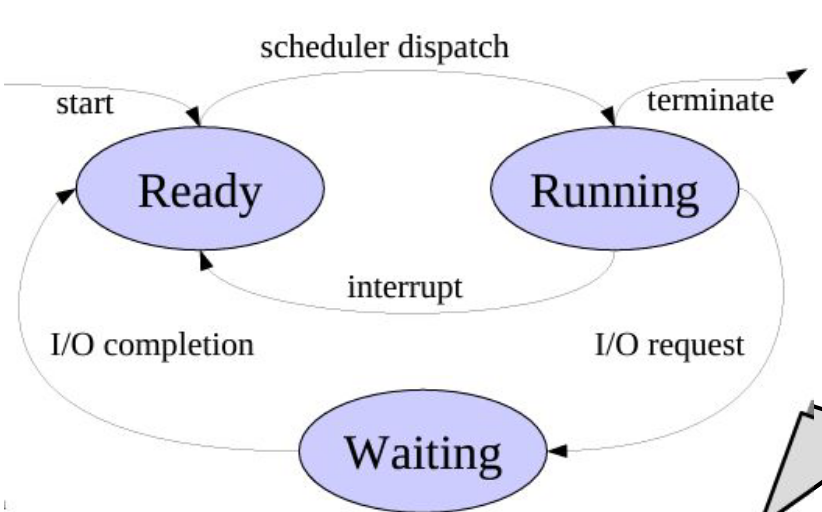
\includegraphics[width=0.5\linewidth]{Images/Screenshot 2024-12-26 at 15-07-23 so-03.1-concorrenza - so-03.1-concorrenza.pdf.png}
\end{figure}

\subsection{Multiprogramming e multiprocessing}

\subsubsection{Cos'è la concorrenza?}

Tema centrale nella progettazione dei S.O. riguarda la gestione
di processi multipli.

Due programmi si dicono in esecuzione concorrente se vengono
eseguiti in parallelo (con parallelismo reale o apparente).
La concorrenza è l'insieme di notazioni per descrivere l'esecuzione concorrente di due o più programmi, sono tecniche per risolvere i problemi associati all'esecuzione concorrente, quali comunicazione e sincronizzazione.
\newline

La multiprogrammazione è stata inventata affinchè più processi
indipendenti condividano il processore. Alcune
applicazioni possono essere progettate come un insieme di processi
o thread concorrenti.

Inoltre, molte funzioni del sistema operativo possono essere implementate come un insieme di processi o thread.

\begin{itemize}
    \item \textbf{Multiprogramming:} più processi su un solo processore, parallelismo apparente.
    \item \textbf{Multiprocessing:} più processi su una macchina con processori multipli, parallelismo reale.
    \item \textbf{Distributed processing:} più processi su un insieme di computer distribuiti e indipendenti, parallelismo reale.
\end{itemize}

\subsubsection{Differenze tra multiprocessing e multiprogramming}
\paragraph{In un singolo processore:}processi multipli sono "alternati nel tempo" per dare l'impressione di
avere un multiprocessore. Ad ogni istante, al massimo un processo è in esecuzione, si parla di \textbf{interleaving}.

\paragraph{In un sistema multiprocessore:}più processi vengono eseguiti simultaneamente su processori diversi, i processi sono "alternati nello spazio e si parla di \textbf{overlapping}.

\paragraph{}
A prima vista si potrebbe pensare che queste differenze comportino
problemi distinti.
In un caso l'esecuzione è simultanea, nell'altro caso la simultaneità è solo simulata.

In realtà presentano gli stessi problemi, ovvero, non è possibile predire la velocità relativa dei processi.

\paragraph{Alcune considerazioni:} non vi è sostanziale differenza tra i problemi relativi a multiprogramming e multiprocessing, ai fini del ragionamento sui programmi concorrenti si ipotizza che sia
presente un "processore ideale" per ogni processo.

I problemi derivano dal fatto che non è possibile predire gli istanti temporali in cui vengono eseguite le istruzioni i due processi quando accedono ad una o più risorse condivise.

\subsubsection{Race condition}
\paragraph{Definizione:}si dice che un sistema di processi multipli presenta una race condition qualora il risultato finale dell'esecuzione dipenda dalla temporizzazione con cui vengono eseguiti i processi.
\paragraph{}
Per scrivere un programma concorrente è necessario eliminare le race condition.
\newline
In pratica scrivere programmi concorrenti è più difficile che scrivere programmi sequenziali.
La correttezza non è solamente determinata dall'esattezza dei passi
svolti da ogni singola componente del programma, ma anche dalle
interazioni (volute o no) tra essi.
Fare debug di applicazioni che presentano race condition non
è per niente piacevole...

\subsubsection{Notazione per descrivere processi concorrenti}

\begin{lstlisting}
    process nome {
... statement(s) ...
}
\end{lstlisting}

Esempio

\begin{lstlisting}
process P1 {
    totale = totale + valore;
}

process P2 {
    totale = totale - valore;
}
\end{lstlisting}

\section{Interazioni tra processi}

E' possibile classificare le modalità di interazione tra processi
in base a quanto sono "consapevoli" l’uno dell'altro.


\subsection{Tipi di interazione}
\subsubsection{Processi ignari}
Processi totalmente "ignari" l’uno dell'altro non sono progettati per lavorare insieme, sebbene siano indipendenti, vivono in un ambiente comune.
\paragraph{Come interagiscono?} essi competono per le stesse risorse e devono sincronizzarsi nella loro utilizzazione. Il sistema operativo ha il compito di arbitrare questa competizione, fornendo meccanismi di sincronizzazione.

\subsubsection{Processi indiretti}
Mentre processi "indirettamente" a conoscenza uno dell'altro
sono processi che condividono risorse, come ad esempio un buffer, al fine di scambiarsi informazioni, non si conoscono in base ai loro id, ma interagiscono indirettamente tramite le risorse condivise.
\paragraph{Come interagiscono?} cooperano per qualche scopo e devono sincronizzarsi nella utilizzazione delle risorse. Il sistema operativo deve facilitare la cooperazione, fornendo meccanismi di sincronizzazione.

\subsubsection{Processi diretti}
Processi "direttamente" a conoscenza uno dell'altro sono coloro che comunicano uno con l'altro sulla base dei loro id, la comunicazione è diretta, spesso basata sullo scambio di messaggi
\paragraph{Come interagiscono?} cooperano per qualche scopo e comunicano informazioni agli altri processi.
Il sistema operativo deve facilitare la cooperazione, fornendo meccanismi di comunicazione.

\subsection{Proprietà fondamentali}
\paragraph{Definizione:}una proprietà di un programma concorrente è un attributo che rimane vero per ogni possibile storia di esecuzione del programma stesso.

Esistono due tipi di proprietà:
\begin{itemize}
    \item \textbf{Safety ("nothing bad happens"): }mostrano che il programma (se avanza) va "nella direzione voluta", cioè
non esegue azioni scorrette.
    \item \textbf{Liveness ("something good eventually happens"): }il programma avanza, non si ferma... insomma è “vitale.
\end{itemize}

Esempio: \textbf{Consensus }
\newline
Si consideri un sistema con N processi: all'inizio, ogni processo propone un valore. Alla fine, tutti i processi si devono accordare su uno dei valori proposti (decidono quel valore).
\newline

\textbf{Proprietà di safety: }se un processo decide, deve decidere uno dei valori proposti, se due processi decidono, devono decidere lo stesso valore.
\newline

\textbf{Proprietà di liveness: } prima o poi ogni processo corretto \textit{(i.e. non in crash)} prenderà una decisione.

\subsubsection{Proprietà - programmi sequenziali}
Nei programmi sequenziali le \textbf{proprietà di safety} esprimono la correttezza dello stato finale (il risultato è quello voluto).
La principale \textbf{proprietà di liveness} è la terminazione.

\subsubsection{Proprietà - programmi concorrenti}
\paragraph{Proprietà di safety:} i processi non devono "interferire" fra di loro nell'accesso alle risorse
condivise, questo vale ovviamente per i processi che condividono risorse (non per processi che cooperano tramite comunicazione).
I meccanismi di sincronizzazione servono a garantire la
proprietà di safety, devono essere usati propriamente dal programmatore, altrimenti il programma potrà contenere delle race conditition.

\paragraph{Proprietà di liveness:} i meccanismi di sincronizzazione utilizzati non devono prevenire l'avanzamento del programma. Non è possibile che tutti i processi si "blocchino", in attesa di eventi che non possono verificarsi perché generabili solo da altri processi bloccati.
Non è possibile che un processo debba "attendere indefinitamente"
prima di poter accedere ad una risorsa condivisa.

\subsection{Mutua esclusione}
\paragraph{Definizione:} l'accesso ad una risorsa si dice mutualmente esclusivo se ad ogni istante, al massimo un processo può accedere a quella risorsa.

\textit{Esempi da considerare: due processi che vogliono accedere contemporaneamente a una stampante. Due processi che cooperano scambiandosi informazioni tramite un buffer condiviso.}

\subsection{Deadlock (stallo)}
La mutua esclusione permette di risolvere il problema della non
interferenza, ma può causare il blocco permanente dei processi.
\newline

Esempio:
Siano $R_1$ e $R_2$ due risorse.
Siano $P_1$ e $P_2$ due processi che devono accedere a $R_1$ e $R_2$ contemporaneamente, prima di poter terminare il programma.

Supponiamo che il S.O. assegni $R_1$ a $P_1$, e $R_2$ a $P_2$
\newline

I due processi sono bloccati in attesa circolare, si dice che $P_1$ e $P_2$ sono in \textbf{deadlock}.
E' una condizione definitiva da evitare.
Nei sistemi reali, se ne può uscire solo con metodi "distruttivi", ovvero uccidendo i processi, riavviando la macchina, etc.

\subsection{Starvation (inedia)}
Il deadlock è un problema che coinvolge tutti i processi che utilizzano un certo insieme di risorse. Esiste anche la possibilità che un processo non possa accedere ad una risorsa perché "sempre occupata".

\textit{Esempio: se siete in coda ad uno sportello e continuano ad arrivare "furbi" che passano davanti, non riuscirete mai a parlare con l'impiegato.}
\newline

Esempio:
Sia R una risorsa.
Siano $P_1$, $P_2$ e $P_3$ tre processi che devono accedere periodicamente a R.
\newline

Supponiamo che $P_1$ e $P _2$ si alternino nell'uso della risorsa
$P_3$ non può accedere alla risorsa, perché utilizzata in modo esclusivo dagli altri due processi.

Si dice che $P_3$ è in \textbf{starvation}.
A differenza del deadlock, non è una condizione definitiva è possibile uscirne, basta adottare un'opportuna politica di assegnamento.
Rimane comunque una situazione da evitare.

\subsection{Azioni atomiche}
\paragraph{Definizione:} le azioni atomiche vengono compiute in modo indivisibile, soddisfano la condizione: o tutto o niente.
Nel caso di parallelismo reale si garantisce che l'azione non interferisca con altri processi durante la sua esecuzione.
Nel caso di parallelismo apparente l'avvicendamento (context switch) fra i processi avviene prima o dopo l'azione, che quindi non può interferire.
\newline

Esempi:
Le singole istruzioni del linguaggio macchina sono atomiche
\begin{lstlisting}
     sw $a0, ($t0)
\end{lstlisting}

\paragraph{Nel caso di parallelismo apparente:}il meccanismo degli interrupt (su cui è basato l'avvicendamento dei processi) garantisce che un interrupt venga eseguito prima o dopo un'istruzione, mai "durante".

\paragraph{Nel caso di parallelismo reale:} anche se più istruzioni cercano di accedere alla stessa cella di
memoria (quella puntata da $t0$), la politica di arbitraggio del bus garantisce che una delle due venga servita per prima e l'altra
successivamente.
\newline

Controesempi:
In generale, sequenze di istruzioni in linguaggio macchina non
sono azioni atomiche
\begin{lstlisting}
    lw $t0, ($a0)
    add $t0, $t0, $a1
    sw $t0, ($a0)
\end{lstlisting}
\textit{(Attenzione però: le singole istruzioni in linguaggio macchina sono atomiche, le singole istruzioni in assembly possono non essere atomiche!)}
\newline

E nei compiti di concorrenza?
Assumiamo che in ogni istante, vi possa essere al massimo un accesso alla memoria alla volta.

Questo significa che operazioni tipo: aggiornamento di una variabile, incremento di una variabile e valutazione di espressioni
\textbf{non sono atomiche}.

Operazioni tipo: assegnamento di un valore costante ad una variabile, \textbf{sono atomiche}.

\subsubsection{Annotazione}
Nel seguito, utilizzeremo la notazione \textbf{$<S>$} per indicare che lo statement S deve essere eseguito in modo atomico
\newline

Esempio:
\begin{lstlisting}
    < x = x + 1; >
\end{lstlisting}

\section{Sezioni critiche}

\subsubsection{Non interferenza}
Se le sequenze di istruzioni non vengono eseguite in modo atomico,
come possiamo garantire la non-interferenza?

Dobbiamo trovare il modo di specificare che certe parti dei programmi sono "speciali", ovvero devono essere eseguite in modo atomico (senza interruzioni).

\paragraph{Definizione:} La parte di un programma che utilizza una o più risorse condivise viene detta \textbf{sezione critica} (critical section, o \textbf{CS}).
\newline

Esempio:
\begin{lstlisting}
    process P1 {
        a1 = rand();
        totale = totale + a1; //CS
    }

    process P2 {
        a2 = rand();
        totale = totale + a2; //CS
}
\end{lstlisting}

La parte evidenziata è una sezione critica, in quanto accede alla
risorsa condivisa totale; mentre a1 e a2 non sono condivise.

\paragraph{Obiettivi:}Vogliamo garantire che le sezioni critiche siano eseguite in modo
mutualmente esclusivo (atomico) evitando così situazioni di blocco, sia dovute a deadlock sia dovute a starvation.

\paragraph{Sintassi:}
\begin{itemize}
    \item \textbf{[enter cs]} indica il punto di inizio di una sezione critica.
    \item \textbf{[exit cs]} indica il punto di fine di una sezione critica.
\end{itemize}

Perché abbiamo bisogno di costrutti specifici? Perché il S.O. non può capire da solo cosa è una sezione critica e cosa non lo è.

Esempio:
\begin{lstlisting}
    x=0
    cobegin
        [enter cs]; x = x+1; [exit cs];

        [enter cs]; x = x+1; [exit cs];
    coend
\end{lstlisting}

\subsubsection{Requisiti delle CS}
Si tratta di realizzare N processi della forma:
\begin{lstlisting}
    process Pi { // i=1...N 
        while (true) {
        [enter cs]
            critical section
        [exit cs]
            non-critical section
        }
    }       
\end{lstlisting}
  
In modo che valgano le seguenti proprietà:
\begin{enumerate}
    \item \textbf{Mutua esclusione:} solo un processo alla volta deve essere all'interno della CS, fra tutti quelli che hanno una CS per la stessa risorsa condivisa.
    \item \textbf{Assenza di deadlock:} uno scenario in cui tutti i processi restano bloccati definitivamente non è ammissibile.
    \item \textbf{Assenza di delay non necessari:} un processo fuori dalla CS non deve ritardare l'ingresso della CS da parte di un altro processo.
    \item \textbf{Eventual entry (assenza di starvation:)} ogni processo che lo richiede, prima o poi entra nella CS.
\end{enumerate}
 \textit{N.B: Se un processo entra in una critical section, prima o poi ne uscirà, quindi esso può terminare solo fuori dalla sua sezione critica!}

 \subsubsection{Possibili approcci}
 \begin{itemize}
    \item \textbf{Approcci software:} la responsabilità cade sui processi che vogliono accedere ad un oggetto distribuito, Può essere soggetto ad errori e vedremo che è costoso in termini di esecuzione (busy waiting).
    \item \textbf{Approcci hardware:} utilizza istruzioni speciali del linguaggio macchina, progettate apposta. Sono efficienti ma non sono adatti come soluzioni general-purpose.
    \item \textbf{Approcci basati su supporto nel S.O. o nel linguaggio:} la responsabilità di garantire la mutua esclusione ricade sul S.O. o sul linguaggio.
    \textit{Esempi: semafori, monitor, message passing.}
 \end{itemize}
\newpage

\subsection{Tecniche software: Algoritmo di Dekker}
\begin{lstlisting}
    shared int turn = P;
    shared boolean needp = false; shared boolean needq = false;
    
    cobegin P -> Q coend
        
        process P {
            while (true) {
                // entry protocol 
                needp = true;
                while (needq)
                    if (turn == Q) {
                        needp = false;
                        while (turn == Q);
                            // do nothing 
                        needp = true;
                    }
                //critical section
                needp = false; turn = Q;
                //non-critical section
            }
        }

        process Q {
            while (true) {
                // entry protocol 
                needq = true;
                while (needp)
                    if (turn == P) {
                        needq = false;
                        while (turn == P); 
                            // do nothing
                        needq = true;
                    }
                //critical section
                needq = false; turn = P;
                //non-critical section
            }
        }
\end{lstlisting}

\subsubsection{Dimostrazione (mutua esclusione)}

Per assurdo supponiamo che P e Q siano in CS contemporaneamente.
Poiché gli accessi in memoria sono esclusivi, per entrare devono almeno aggiornare / valutare entrambe le variabili needp e needq.

Uno dei due entra per primo; diciamo sia Q: needq sarà true fino a quando Q non uscirà dal ciclo, poiché P entra nella CS mentre Q è nella CS, significa che esiste un istante temporale in cui needq = false e Q è in CS.
\newline
ASSURDO!

\subsubsection{Dimostrazione (assenza di deadlock)}
Per assurdo supponiamo che né P né Q possano entrare in CS. P e Q devono essere bloccati nel primo while, esiste un istante t dopo di che needp e needq sono sempre true.

Supponiamo che all'istante t, turn = Q.
L'unica modifica a turn può avvenire solo quando Q entra in CS, dopo t, turn resterà sempre uguale a Q, P entra nel primo ciclo, e mette needp = false.
\newline
ASSURDO!

\subsubsection{Dimostrazione (assenza di ritardi non necessari)}
Se Q sta eseguendo codice non critico, allora needq = false.
Allora P può entrare nella CS.

\subsubsection{Dimostrazione (assenza di starvation)}
Se Q richiede di accedere alla CS: needq = true.
Se P sta eseguendo codice non critico: Q entra
Se P sta eseguendo il resto del codice (CS, entrata, uscita): prima o poi ne uscirà e metterà il turno a Q.
Q potrà quindi entrare.

\subsection{Tecniche software: Algoritmo di Peterson}
Più semplice e lineare di quello di Dijkstra / Dekker
e facilmente generalizzabile al caso di processi multipli.

\begin{lstlisting}
    shared boolean needp = false;
    shared boolean needq = false;
    shared int turn;
    
    cobegin P -> Q coend
        
        process P {
            while (true) {
                // entry protocol
                needp = true;
                turn = Q;
                while (needq && turn != P); 
                    // do nothing
                //critical section
                needp = false;
                //non-critical section
            }
        }

        process Q {
            while (true) {
                // entry protocol
                needq = true;
                turn = P;
                while (needp && turn != Q);
                    //do nothing
                //critical section
                needq = false;
                //non-critical section
            }
        }
\end{lstlisting}

\subsubsection{Dimostrazione (mutua esclusione)}
Supponiamo che P sia entrato nella sezione critica.

Vogliamo provare che Q non può entrare, sappiamo che needP == true
e Q entra solo se turn = Q quando esegue il while.
Si consideri lo stato al momento in cui P entra nella critical section.

Ho due possibilità, needq == false or turn == P:
\begin{itemize}
    \item Se needq == false, Q doveva ancora eseguire needq == true, e quindi lo eseguirà dopo l'ingresso di P e porrà turn=P, precludendosi la possibilità di entrare.
    \item Se turn==P, come sopra;
\end{itemize}




\subsubsection{Dimostrazione (assenza di deadlock)}

Supponiamo che per assurdo che P voglia entrare nella CS e sia
bloccato nel suo ciclo while, questo significa che: needp = true, needq = true, turn = Q per sempre.

Possono darsi tre casi:
\begin{itemize}
    \item Q non vuole entrare in CS: impossibile, visto che needq = true
    \item Q è bloccato nel suo ciclo while: impossibile, visto che turn = Q
    \item Q è nella sua CS e ne esce (prima o poi): impossibile, visto che prima o poi needq assumerebbe il valore false
\end{itemize}

\subsubsection{Dimostrazione (assenza di ritardi non necessari)}
Se Q sta eseguendo codice non critico, allora needq = false, allora P può entrare nella CS.

\subsubsection{Dimostrazione (assenza di starvation)}
Simile alla dimostrazione di assenza di deadlock, aggiungiamo un caso in fondo:
Q continua ad entrare ed uscire dalla sua CS, prevenendo l'ingresso di P.

Impossibile poiché quando Q prova ad entrare nella CS pone turn = P
siccome needp = true e  quindi Q deve attendere che P entri nella CS.

\subsection{Algoritmo di Peterson – Generalizzazione per N processi}

\begin{lstlisting}
    shared int[] stage = new int[N]; /* 0-initialized */
    shared int[] last = new int[N]; /* 0-initialized */
    
    cobegin P0 -> P1 -> ... -> PN-1 coend

    process Pi { // i = 0...N-1 
        while (true) {
        // Entry protocol
        for (int j=0; j < N; j++) {
            stage[i] = j; last[j] = i;
            for (int k=0; k < N; k++) {
                if (i != k){
                    while (stage[k] >= stage[i] && last[j] == i)
                    ;
                    }
                }
        }
        //critical section
        stage[i] = 0;
        //non-critical section
        }
    }
\end{lstlisting}



\subsection{Tecniche hardware: disabilitazione interrupt, istruzioni speciali}
Le soluzioni di Dekker e Peterson prevedono come uniche istruzioni
atomiche le operazioni di Load e Store. Si può pensare di fornire alcune istruzioni hardware speciali per semplificare la realizzazione di sezioni critiche.
Nei sistemi uniprocessore, i processi concorrenti vengono "alternati" tramite il meccanismo degli interrupt.
Possiamo quindi disabilitarli.
\newline

\textit{Esempio:}

\begin{lstlisting}
    process P {
        while (true) {
            //disable interrupt
            critical section

            //enable interrupt
            non-critical section
        }
    }
\end{lstlisting}

Il problema è che il S.O. deve lasciare ai processi la responsabilità di riattivare gli interrupt ciò è altamente pericoloso perchè riduce il grado di parallelismo ottenibile dal processore. Inoltre non funziona su sistemi multiprocessore.
\newpage

\subsubsection{Test e Set}
Test e Set sono istruzioni che realizzano due azioni in modo atomico.
\textit{Esempi: lettura e scrittura, test e scrittura.}

$TS(x,y) := < y = x ; x = 1 >$
\newline
Esso ritorna in y il valore precedente di x e assegna 1 ad x.

\begin{lstlisting}
    shared lock=0; cobegin P -> Q coend
    
    process P {
        int vp;
        while (true) {
            do {
                TS(lock, vp);
            } while (vp);
            
            //critical section
            lock=0;
            //non-critical section
        }
    }

    process Q {
        int vp;
        while (true) {
            do {
                TS(lock, vp);
            } while (vp);
            
            //critical section
            lock=0;
            //non-critical section
        }
    }
\end{lstlisting}

\paragraph{Rispetta tutti i requisiti delle CS:}
\begin{itemize}
    \item Mutua esclusione: entra solo chi riesce a settare per primo il lock.
    \item No deadlock: il primo che esegue TS entra senza problemi.
    \item No unnecessary delay: un processo fuori dalla CS non blocca gli altri.
    \item No starvation: no, se non assumiamo qualcosa di più.
\end{itemize}

\subsubsection{Riassumendo}
\begin{itemize}
    \item \textbf{Vantaggi delle istruzioni speciali hardware:}
    \begin{itemize}
        \item sono applicabili a qualsiasi numero di processi, sia su sistemi monoprocessore che in sistemi multiprocessori.
        \item semplice e facile da verificare.
        \item può essere utilizzato per supportare sezioni critiche multiple; ogni sezione critica può essere definita dalla propria variabile.
    \end{itemize}
    \item \textbf{Svantaggi:}
    \begin{itemize}
        \item si utilizza ancora busy-waiting.
        \item i problemi di starvation non sono eliminati.
        \item sono comunque complesse da programmare.
    \end{itemize}
\end{itemize}

\section{Semafori}
Due o più processi possono cooperare attraverso semplici segnali, in modo tale che un processo possa essere bloccato in specifici punti del suo programma finché non riceve un segnale da un altro processo.

\subsection{Definizione}
E' un tipo di dato astratto per il quale sono definite due operazioni:
\begin{itemize}
    \item  \textbf{V} (dall'olandese verhogen): viene invocata per inviare un segnale, quale il verificarsi di un evento o il rilascio di una risorsa.
    \item  \textbf{P} (dall'olandese proberen): viene invocata per attendere il segnale (ovvero, per attendere un evento o il rilascio di una risorsa).
\end{itemize}

Un semaforo può essere visto come una variabile intera, che viene inizializzata ad un valore non negativo.
L'operazione P attende che il valore del semaforo sia positivo e decrementa il valore del semaforo.
L'operazione V incrementa il valore del semaforo.

\textit{N.B: le azioni P e V sono atomiche}

\begin{lstlisting}
    class Semaphore {
    private int val;
    Semaphore(int init) { }
        void P() {}
        void V() {}
}
\end{lstlisting}

\subsubsection{Semaforo - Invariante}

Siano:
\begin{itemize}
    \item $n_P$ il numero di operazioni P completate
    \item $n_V$ il numero di operazioni V completate
    \item init il valore iniziale del semaforo
\end{itemize}

Vale il seguente invariante: $n_P \leq n_V + init$

Due casi:
\begin{itemize}
    \item \textbf{eventi ($init = 0$)} : il numero di eventi "consegnati" deve essere non superiore al numero di volte che l'evento si è verificato.
    \item \textbf{risorse ($init \geq 0$)} : il numero di richieste soddisfatte non deve essere superiore al numero iniziale di risorse + il numero di risorse restituite.
\end{itemize}

\subsubsection{Implemetazione di CS}
\begin{lstlisting}
    Semaphore s = new Semaphore(1);

        process P {
            while (true) {
                s.P();
                //critical section
                s.V();
                //non-critical section
            }
        }
\end{lstlisting}

\subsubsection{Politiche di gestione dei processi bloccati}
Per ogni semaforo, il S.O. deve mantenere una struttura dati contenente l'insieme dei processi sospesi. Quando un processo deve essere svegliato, è necessario selezionare uno dei processi sospesi.

I \textbf{semafori FIFO} adottano la politica first-in, first-out.
Il processo che è stato sospeso più a lungo viene svegliato per primo, è una politica fair, che garantisce assenza di starvation, la struttura dati è una coda.
Se non viene specificata l'ordine in cui vengono rimossi, i semafori possono dare origine a starvation.
\newline

Da ora in poi utilizzeremo solo i semafori FIFO...
\newpage

\subsection{Implementazione}

\subsubsection{La funzione P}

\begin{lstlisting}
    void P() {
        value--;
        if (value < 0) {
            pid = <id del processo che ha invocato P>;
            queue.add(pid);
            suspend(pid);
        }
    }
\end{lstlisting}    

\textbf{Riga 5} Il process id del processo bloccato viene messo in un insieme queue.

\textbf{Riga 6} Con l'operazione suspend, il s.o mette il processo nello stato waiting.

\subsubsection{La funzione V}

\begin{lstlisting}
    void V() {
        value++;
        if (value <= 0){
            pid = queue.remove();
            wakeup(pid);
        }
    }
\end{lstlisting}

\textbf{Riga 4} Il process id del processo da sbloccare viene selezionato dall'insieme queue.

\textbf{Riga 5} Con l'operazione wakeup, il S.O. mette il processo nello stato ready.
\newline

Quindi è necessario utilizzare una delle tecniche di critical section viste in precedenza: Dekker, Peterson oppure test-set, swap, etc.

\begin{lstlisting}
    void P() {
        //[enter CS]
        value--;
        if (value < 0) {
            int pid = <id del processo che ha invocato P>;
            queue.add(pid);
            suspend(pid);
        }
        //[exit CS]
    }
    

    void V() {
        //[enter CS]
        value++;
        if (value <= 0){
            int pid = queue.remove();
            wakeup(pid);
        }
        //[exit CS]
    }
\end{lstlisting}

Utilizzando queste tecniche, abbiamo limitato busy-waiting alle sezioni critiche di P e V, e queste sezioni critiche sono molto brevi, in questo modo la sezione critica non è quasi mai occupata
e busy waiting avviene raramente.

\subsection{Semafori binari}

\paragraph{Definizione:}variante dei semafori in cui il valore può assumere solo i valori 0 e 1.

\paragraph{A cosa servono?}servono a garantire mutua esclusione, semplificando il lavoro del programmatore.
Hanno lo stesso potere espressivo dei semafori "normali".

\paragraph{Invariante dei semafori binari:}
$0 \leq n_V + init - n_P \leq 1$ oppure $0 \leq s.value \leq 1$
\newpage

\subsubsection{Implementazione nei sistemi operativi}
\begin{lstlisting}
    class BinarySemaphore {
        private int value;
        Queue queue0 = new Queue();
        Queue queue1 = new Queue();
        BinarySemaphore() { value = 1; }

        void P() {
            //[enter CS]
            int pid = <process id>;
            if (value == 0) {
                queue0.add(pid);
                suspend(pid);
            }
            value--;
        
            if (queue1.size() > 0) {
                int pid = queue1.remove();
                wakeup(pid);
            }
            //[exit CS]
        }

        void V() {
            //[enter CS]
            int pid = <process id>;
            if (value == 1) {
                queue1.add(pid);
                suspend(pid);
            }
            value++;
            
            if (queue0.size() > 0) {
                int pid = queue0.remove();
                wakeup(pid);
            }
            //[exit CS]
        }
\end{lstlisting}

\subsubsection{Implementazione tramite semafori generali}
\begin{lstlisting}
    class BinarySemaphore {
        private Semaphore s0 , s1 ;
        int value ;

        BinarySemaphore(int v){ //fail if v not in {0,1}
            s0 = new Semaphore(v)
            s1 = new Semaphore(1-v)
        }
        
        void P(void){
            s0.P();
            s1.V();
        }

        void V(void){
            s1.P();
            s0.V();
        }
    }
\end{lstlisting}

\section{Problemi classici}
Esistono un certo numero di problemi "classici" della programmazione concorrente:
\begin{itemize}
    \item producer/consumer
    \item bounded buffer
    \item dining philosophers
    \item readers/writers
\end{itemize}

Nella loro semplicità rappresentano le interazioni tipiche dei processi concorrenti.

\subsection{Producer/Consumer}

\paragraph{Definizione:} esiste un processo "produttore" \textbf{Producer} che genera valori (record, caratteri, oggetti, etc.) e vuole trasferirli a un processo "consumatore" \textbf{Consumer} che prende i valori generati e li "consuma".
La comunicazione avviene attraverso una singola variabile condivisa.

\paragraph{Proprietà da garantire:} Producer non deve scrivere nuovamente l'area di memoria condivisa prima che Consumer abbia effettivamente utilizzato il valore precedente.
Consumer non deve leggere due volte lo stesso valore, ma deve attendere che Producer abbia generato il successivo.
Assenza di deadlock.

\begin{lstlisting}
    shared Object buffer;
    Semaphore empty = new Semaphore(1);
    Semaphore full = new Semaphore(0);

    //cobegin
        Producer
        ....
        Consumer
    //coend

    process Producer {
        while (true) {
            Object val = produce();
            empty.P();
            buffer = val;
            full.V();
        }
    }
    
    process Consumer {
        while (true) {
            full.P();
            Object val = buffer;
            empty.V();
            consume(val);
        }
    }

\end{lstlisting}


\subsection{Bounded Buffer}
\paragraph{Definizione:} è simile al problema del produttore/consumatore.
In questo caso, però, lo scambio tra produttore e consumatore non
avviene tramite un singolo elemento, ma tramite un buffer di
dimensione limitata, i.e. un vettore di elementi.
\paragraph{Proprietà da garantire:} Producer non deve sovrascrivere elementi del buffer prima che Consumer abbia effettivamente utilizzato i relativi valori.
Consumer non deve leggere due volte lo stesso valore, ma deve
attendere che Producer abbia generato il successivo.
Assenza di deadlock e assenza di starvation.

\subsubsection{Struttura del buffer}
Array circolare: si utilizzano due indici front e rear che indicano rispettivamente il prossimo elemento da scrivere e il prossimo elemento da leggere. Gli indici vengono utilizzati in modo ciclico (modulo l'ampiezza del buffer).

\textit{Esempi:}
\begin{figure} [h]
    \centering
    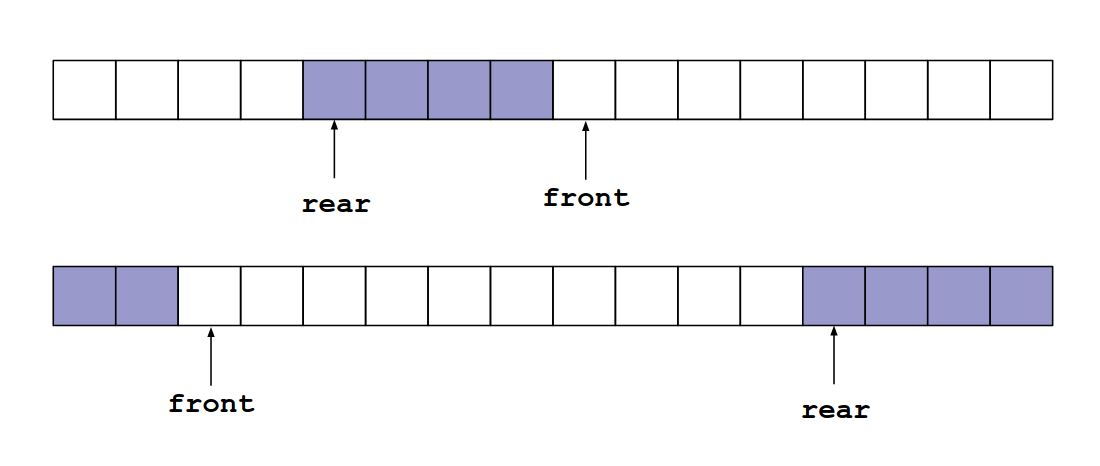
\includegraphics[width=0.5\linewidth]{Images/Screenshot 2024-12-28 at 19-31-02 so-03.1-concorrenza - so-03.1-concorrenza.pdf.png}
\end{figure}

\begin{lstlisting}
    Object buffer[SIZE];
    int front = 0;
    int rear = 0;
    Semaphore empty = new Semaphore(SIZE);
    Semaphore full = new Semaphore(0);

    process Producer {
        while (true) {
            Object val = produce();
            empty.P();
            buf[front] = val;
            front = (front + 1) % SIZE;
            full.V();
        }
    }

    process Consumer {
        while (true) {
            full.P();
            Object val = buf[rear];
            rear = (rear + 1) % SIZE;
            empty.V();
            consume(val);
        }
    }
\end{lstlisting}

\subsection{Cena dei Filosofi}
\paragraph{Descrizione:}Cinque filosofi passano la loro vita a pensare e a mangiare (alternativamente).
Per mangiare fanno uso di una tavola rotonda con 5 sedie, 5 piatti e 5 posate fra i piatti.
Per mangiare, un filosofo ha bisogno di entrambe le posate (destra/sinistra), per pensare, un filosofo lascia le posate
dove le ha prese.

I problemi produttore/consumatore e buffer limitato mostrano come risolvere il problema di accesso esclusivo a una o più
risorse indipendenti.

Il problema dei filosofi mostra come gestire situazioni in cui i processi entrano in competizione per accedere ad insiemi di risorse a intersezione non nulla.

\subsubsection{La vita di un filosofo}
\begin{lstlisting}
    process Philo[i] { /* i = 0...4 */
        while (true) {
            //think
            //acquire chopsticks
            //eat
            //release chopsticks
        }
    }
\end{lstlisting}        

Le bacchette vengono denominate: \textbf{chopstick[i]} con i=0...4;
Il filosofo i accede alle posate chopstick[i] e chopstick[(i+1) \% 5];
\subsubsection{Invarianti}
$up_i$ il numero di volte che la bacchetta i viene preso dal tavolo
$down_i$ il numero di volte che la bacchetta i viene rilasciata sul tavolo
\newpage
\textbf{Invariante}
$down_i \leq up_i \leq down_i + 1$

Per comodità si può definire chopstick[i] = 1 - ($up_i-down_i$)
(può essere pensato come un semaforo binario)

\subsubsection{Soluzione}
\begin{lstlisting}
Semaphore chopsticks = { new Semaphore(1), ..., new Semaphore(1)};

    process Philo[0] {
        while (true) {
            //think
            chopstick[1].P();
            chopstick[0].P();
            //eat
            chopstick[1].V();
            chopstick[0].V();
        }
    }

    process Philo[i] { /* i = 1...4 */
        while (true) {
            //think
            chopstick[i].P();
            chopstick[(i+1)%5].P();
            //eat
            chopstick[i].V();
            chopstick[(i+1)%5].V();
        }
    }
\end{lstlisting}

\subsection{Lettori e scrittori}

\paragraph{Descrizione:} Un database è condiviso tra un certo numero di processi, esistono due tipi di processi.
I lettori accedono al database per leggerne il contenuto
e gli scrittori accedono al database per aggiornarne il contenuto.

\paragraph{Proprietà:} Se uno scrittore accede a un database per aggiornarlo, esso opera in mutua esclusione; nessun altro lettore o scrittore può accedere al database.
Se nessuno scrittore sta accedendo al database, un numero arbitrario di lettori può accedere al database in lettura.

\paragraph{Motivazioni:} La competizione per le risorse avviene a livello di classi di processi e non solo a livello di processi. Mostra che mutua esclusione e condivisione possono anche coesistere.

\paragraph{Invariante:} Sia \textbf{nr} il numero dei lettori che stanno accendo al database e sia \textbf{nw} il numero di scrittori che stanno accedendo al database.

L'invariante è il seguente: ($nr > 0$ \&\& $nw == 0$) $||$ ($nr == 0$ \&\& $nw \le 1$)

NOTA: il controllo può passare dai lettori agli scrittori o viceversa quando: $nr == 0$ \&\& $nw == 0$

\begin{lstlisting}
process Reader {
    while (true) {
        startRead();
        //read the database
        endRead();
    }
}

process Writer {
    while (true) {
        startWrite();
        //write the database
        endWrite();
    }
}
\end{lstlisting}

Note: startRead() e endRead() contengono le operazioni
necessarie affinché un lettore ottenga accesso al database.

startWrite() e endWrite() contengono le operazioni necessarie affinchè uno scrittore ottenga accesso al database.

\paragraph{}
Il problema dei lettori e scrittori ha molte varianti che si basano sui diversi concetti di priorità.

\subparagraph{Priorità ai lettori} Se un lettore vuole accedere al database, lo potrà fare senza attesa a
meno che uno scrittore non abbia già acquisito l'accesso al database. 

Scrittori hanno possibilità di starvation.
\subparagraph{Priorità agli scrittori} Uno scrittore attenderà il minimo tempo possibile prima di accedere al db.

Lettori hanno possibilità di starvation.

\subsubsection{Lettori e scrittori - Soluzione}

\begin{lstlisting}
/* Variabili condivise */
    int nr = 0;
    Semaphore rw = new
    Semaphore(1);
    Semaphore mutex = new
    Semaphore(1);

    void startRead() {
        mutex.P();
        if (nr == 0){
            rw.P();
            nr++;
            mutex.V();
        }
        void startWrite() {
        rw.P();
    }

    void endRead() {
        mutex.P();
        nr--;
        if (nr == 0) {
            rw.V();
            mutex.V();
        }

    void endWrite() {
        rw.V();
    }
\end{lstlisting}

Problemi: limitata a priorità per i lettori, di comprensione non semplice, non è chiaro da dove saltano fuori alcuni punti della soluzione.

\subsection{Come derivare una soluzione basata su semafori}
\subsubsection{Alcune definizioni utili - Andrews}
Sia \textbf{B} una \textbf{condizione booleana}.

Sia \textbf{S} uno \textbf{statement} (possibilmente composto)

Allora:
$< S >$ : esegui lo statement S in modo atomico.

$< await(B) \rightarrow S>$: attendi fino a che la condizione B è verificata e quindi esegui S. L'attesa e il comando vengono eseguiti in modo atomico, quindi, quando S viene eseguito, B è verificata.

\paragraph{Passi da seguire:}
\begin{enumerate}
    \item Definire il problema con precisione: identificare i processi, specificare i problemi di sincronizzazione, introdurre le variabili necessarie e definire un'invariante.
    \item Abbozzare una soluzione: produrre un primo schema di soluzione, e identificare le regioni che richiedono accesso atomico o mutualmente esclusivo.
    \item Garantire l'invariante: verifica che l'invariante sia sempre verificato
    \item Implementare le azioni atomiche: esprimere le azioni atomiche e gli statement \textbf{await} utilizzando le primitive di sincronizzazione disponibili.
\end{enumerate}

\subsubsection{Soluzione Lettori/Scrittori con Andrews}

\textbf{Variabili:} nr, nw - numero corrente di lettori/scrittori.
\newline
\textbf{Invariante:} ($nr > 0$ \&\& $nw == 0$) $||$ ($nr == 0$ \&\& $nw \le 1$)
\newline
\textbf{Schema della soluzione:}
\begin{lstlisting}
process Reader {
    < await (nw == 0) = nr++ >
    //read the database
    <nr-->
}

process Writer {
    < await (nr == 0 && nw == 0) = nw++ >
    //write the database
    <nw-->
}
\end{lstlisting}

dalla slide 142 alla 155 guardare sulle slide






\section{Conditional Critical Regions (CCR)}
\subsection{Introduzione}
I linguaggi di programmazione concorrente sono dotati di costrutti ad alto livello, che si propongono di prevenire la
possibilità di errori dovuti all'uso scorretto delle primitive.

I costrutti di programmazione concorrente sottraggono al programmatore la responsabilità dell'uso delle primitive
limitando così la possibilità di accessi indiscriminati ai dati comuni e favorendo la programmazione strutturata.

Questo è il compito del compilatore del linguaggio concorrente, che traduce i costrutti per la concorrenza in un insieme di primitive per la concorrenza.

Le \textbf{regioni critiche condizionali} sono costrutti che specificano operazioni su dati condivisi, da eseguire
in mutua esclusione, che possono determinare la sospensione e la riattivazione dei processi.

Forniscono una notazione più strutturata di quella dei semafori per specificare la sincronizzazione.

\subsubsection{Sintassi CCR} 

\lstinline{name (var declarations)}

\textbf{name} è un'identificatore per la risorsa condivisa.

\textbf{var declarations} è un'insieme di variabili condivise.
Dichiara che le variabili racchiuse tra parentesi sono condivise e devono essere accedute in mutua esclusione.

\lstinline{region name when condition do statement}
\textbf{condition} è una condizione booleana.
\lstinline{region name do statement}
\textbf{statement} è uno statement (potenzialmente composto) da eseguire. E' l'istruzione per acquisire la mutua esclusione su name.



\paragraph{L'esecuzione consiste in:}
\begin{itemize}
    \item Acquisire la mutua esclusione
    \item Valutare la condizione:
        \begin{itemize}
            \item se è falsa, rilasciare la mutua esclusione e ritardare fino a quando la condizione non è vera.
            \item se è vera, eseguire statement.
        \end{itemize}
\end{itemize}

\subsubsection{Vantaggi CCR}
Il compilatore del linguaggio attraverso il controllo dello scope delle variabili, può rilevare eventuali riferimenti illegittimi ai dati comuni.

\textit{Esempio: riferimenti non inclusi in regioni critiche condizionali associate al nome corretto}

Inoltre: "Compila" i costrutti region tramite le opportune chiamate a primitive di sincronizzazione (ad. es., semafori)

\subsubsection{Implementazione CCR tramite semafori}
Il ritardo di un processo che, all'interno della CCR, trovi la condizione falsa è realizzata con la sospensione fuori dalla mutua esclusione.

Una tecnica per rilevare la transizione al valore vero della condizione consiste nel far ripetere la verifica della condizione al processo medesimo, che naturalmente deve ri-accedere alla mutua esclusione.

\begin{lstlisting}
    resource name (var declarations)

/* Mutual exclusion semaphore, one for each critical region */
Semaphore mutex_name = new Semaphore(1);
/* Processes for which the condition is false must be
suspended */

Semaphore suspended_name = new Semaphore(0);
/* Number of suspended processes */
int nsuspended_name = 0;
/* Additional declarations */
var declarations
\end{lstlisting}

\begin{lstlisting}
    region name when condition do statement

    mutex_name.P();
    while (!condition) {
        /* condition is false */
        nsuspended_name++;
        mutex_name.V();
        suspended_name.P();
/* when process is reactived, it must re-gain access to the mutual exclusion */
        mutex_name.P();
    }

/* condition is true */
    statement;
/* after statement, one or more conditions may be true */
    while (nsuspended_name-- > 0)
        suspended_name.V();
\end{lstlisting}
\subsubsection{Schema CCR-Semafori}
\begin{figure} [h]
    \centering
    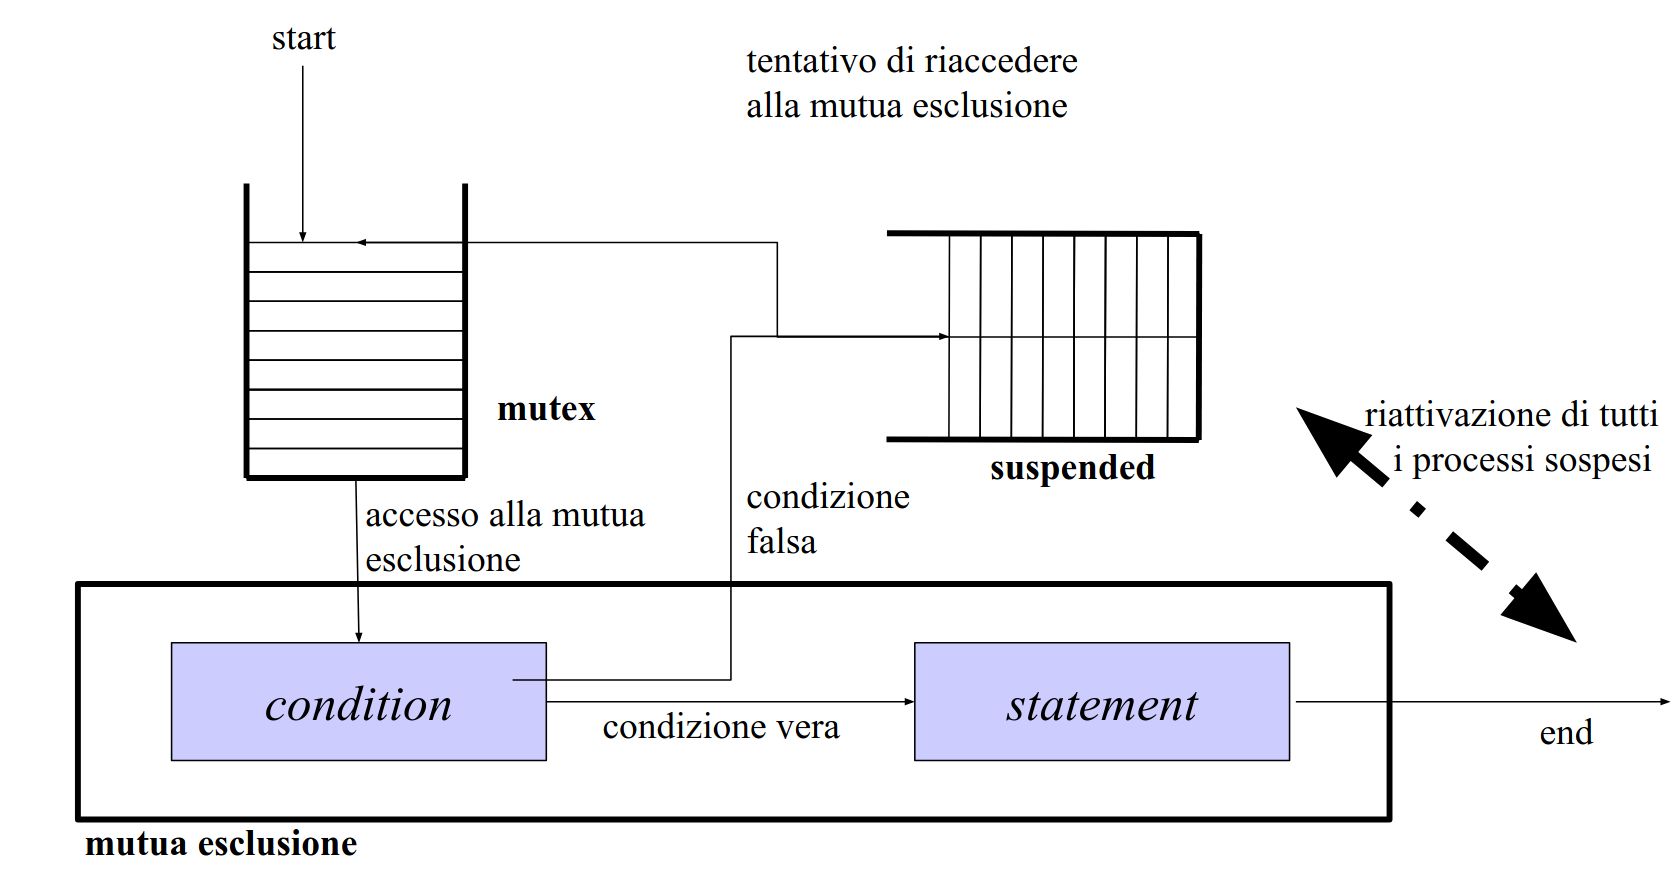
\includegraphics[width=0.85\linewidth]{Images/Screenshot 2025-01-16 at 12-03-09 so-03.1-concorrenza - so-03.1-concorrenza.pdf.png}
\end{figure}

\paragraph{Svantaggi:} questa realizzazione può risultare molto inefficiente nei sistemi uniprocessore, infatti, i processi possono essere riattivati ripetutamente prima di trovare la condizione vera.
Numerosi context switch del tutto improduttivi.

\paragraph{Vantaggi:} è più facile da realizzare qualora le condizioni siano complesse e coinvolgano variabili locali \textit{(non condivise)} dei processi coinvolti.

\subsection{CCR tramite semafori (passing the baton)}
\begin{lstlisting}
resource name (var declarations)

    Semaphore mutex_name = new Semaphore(1);
    Semaphore suspended_name[M_name] = { new Semaphore(0), ..., new Semaphore(0) };

    int nsuspended_name[M_name] = { 0, ..., 0 };
    //var declarations
\end{lstlisting}
dove $M_{name}$ è il numero di regioni critiche con condizione associate a \textbf{name.}

\begin{lstlisting}
region name when condition_i do statement

    mutex_name.P();
    if (!condition_i) {
        nsuspended_name[i]++;
        mutex_name.V();
        suspended_name[i].P();
    }
    statement;
    SIGNAL();


    void SIGNAL() {
        if (nsuspended_name[0] > 0 && condition_0)
            { nsuspended_name[0]--; suspended_name[0].V(); }

        else if (nsuspended_name[1] > 0 && condition_1)
            { nsuspended_name[0]--; suspended_name[1].V(); }

        else if (...)
            ...
        else
            mutex_name.V();
    }
\end{lstlisting}

\subsection{Implementazione di semafori tramite CCR}
Semaforo generali; valore iniziale n
\begin{lstlisting}
class Semaphore {
    resource sem ( int value; );

    Semaphore(int n) {
        /* Initialization; done only once */
        region sem do value = n;
    }

    P() {
        region sem when (value>0) do value--;
    }

    V() {
        region sem do value++;
    }
}
\end{lstlisting}

\subsection{CCR - Produttore / Consumatore}
\begin{lstlisting}
resource buffer (Object b; boolean full = false);

    process Producer {
        while (true) {
        Object val = produce();
        region buffer when (!full) do { b = val; full = true; }
        }
    }

    process Consumer {
        while (true) {
            Object val;
            region buffer when (full) do { val = b; full = false; }
            consume(val);
        }
    }
\end{lstlisting}

\subsection{CCR - Filosofi a cena}
\begin{lstlisting}
    resource table ( 
    boolean eating[N]= { false, false, false, false, false }
    )

    process Philo[i] {
        while (true) {
            //think
            int left = (i+N-1) % N;
            int right = (i+1) % N;
            region table when (!eating[left] && !eating[right]) do

            eating[i] = true;
            //eat
            region table do eating[i] = false;
        }
    }
\end{lstlisting}

\subsection{CCR - R/W Priorità ai lettori}
\begin{lstlisting}
resource db ( int nr = 0; int nw = 0; );

    process Reader {
        while (true) {
            region db when (nw==0) do nr++;
            //read the database
            region db do nr--;
        }
    }

    process Writer {
        while (true) {
            region db when (nr==0 && nw==0) do nw++;
            //write the database
            region db do nw--;
        }
    }
\end{lstlisting}
\newpage
\subsection{CCR - R/W Priorità agli scrittori}
\begin{lstlisting}
resource db ( int nr = 0; int nw = 0; int ww = 0; );

    process Reader {
        while (true) {
            region db when (nw==0 && ww=0) do nr++;
            //read the database
            region db do nr--;
        }
    }

    process Writer {
        while (true) {
            region db do ww++;
            region db when (nr==0 && nw==0) do { nw++; ww--; }
            //write the database
            region db do nw--;
        }
    }
\end{lstlisting}
\subsection{CCR - Bounded buffer (accesso esclusivo)}
\begin{lstlisting}
    resource buffer (
        Object buf[N];
        int front=0; int rear=0;
        int count=0;
    );
    
    process Producer {
        while (true) {
            Object val = produce();
            region buffer
            when (count < N) do {
                buf[front] = val;
                front = (front+1) % N;
                count++;
            }
        }
    }

    process Consumer {
        Object val;
        while (true) {
            region buffer
            when (count > 0) do {
                val = buf[rear];
                rear = (rear+1) % N;
                count--;
            }
            consume(val);
        }
    }
\end{lstlisting}

\newpage
\section{Monitor}
\subsection{Introduzione}
I monitor sono un paradigma di programmazione concorrente che fornisce un approccio più strutturato alla programmazione concorrente.

Un monitor è un modulo software che consiste di: dati locali, una sequenza di inizializzazione e una o più "procedure".

Le caratteristiche principali sono:
\begin{itemize}
    \item I dati locali sono accessibili solo alle procedure del modulo stesso.
    \item Un processo entra in un monitor invocando una delle sue procedure.
    \item Solo un processo alla volta può essere all'interno del monitor; gli altri processi che invocano il monitor sono sospesi, in attesa che il monitor diventi disponibile.
\end{itemize}

\begin{lstlisting}
monitor name {
    
    //private variable declarations...

    procedure entry type procedurename1(args...) {
    //visible procedures 
    }

    type procedurename2(args...) {
    //private procedures
    }

    name(args...) {
    //initialization
    }
}
\end{lstlisting}

Assomiglia ad un "oggetto" nella programmazione Object Oriented, il codice di inizializzazione corrisponde al costruttore.

Le procedure entry sono richiamabili dall'esterno e corrispondono ai metodi pubblici di un oggetto.

Le procedure "normali" corrispondono ai metodi privati.
Le variabili locali corrispondono alle variabili pubbliche.

\subsubsection{Caratteristiche}
Solo un processo alla volta può essere all'interno del monitor, esso fornisce un semplice meccanismo di mutua esclusione. Strutture dati condivise possono essere messe all'interno del monitor.

Per essere utile per la programmazione concorrente, è necessario un meccanismo di sincronizzazione.
Abbiamo quindi necessità di poter sospendere i processi in attesi di qualche condizione, far uscire i processi dalla mutua esclusione mentre sono in attesa e permettergli di rientrare quando la condizione è verificata.

\subsubsection{Meccanismi di sincronizzazione}
Dichiarazione di variabili di condizione (\textbf{CV})
\lstinline{condition c;}
Le operazioni definite sulle CV sono:
\begin{itemize}
    \item \lstinline{c.wait()} - attende il verificarsi della condizione. Viene rilasciata la mutua esclusione, il processo che chiama c.wait() viene sospeso in una coda di
attesa della condizione c.
    \item \lstinline{c.signal()} - segnala che la condizione è vera. Causa la riattivazione immediata di un processo
(secondo una politica FIFO), il chiamante viene posto in attesa e verrà riattivato quando il processo risvegliato avrà rilasciato la mutua esclusione (urgent stack). Se nessun processo sta attendendo c la chiamata non avrà nessun effetto.
\end{itemize}
\newpage
\subsubsection{Rappresentazione grafica} 
\begin{figure} [h]
    \centering
    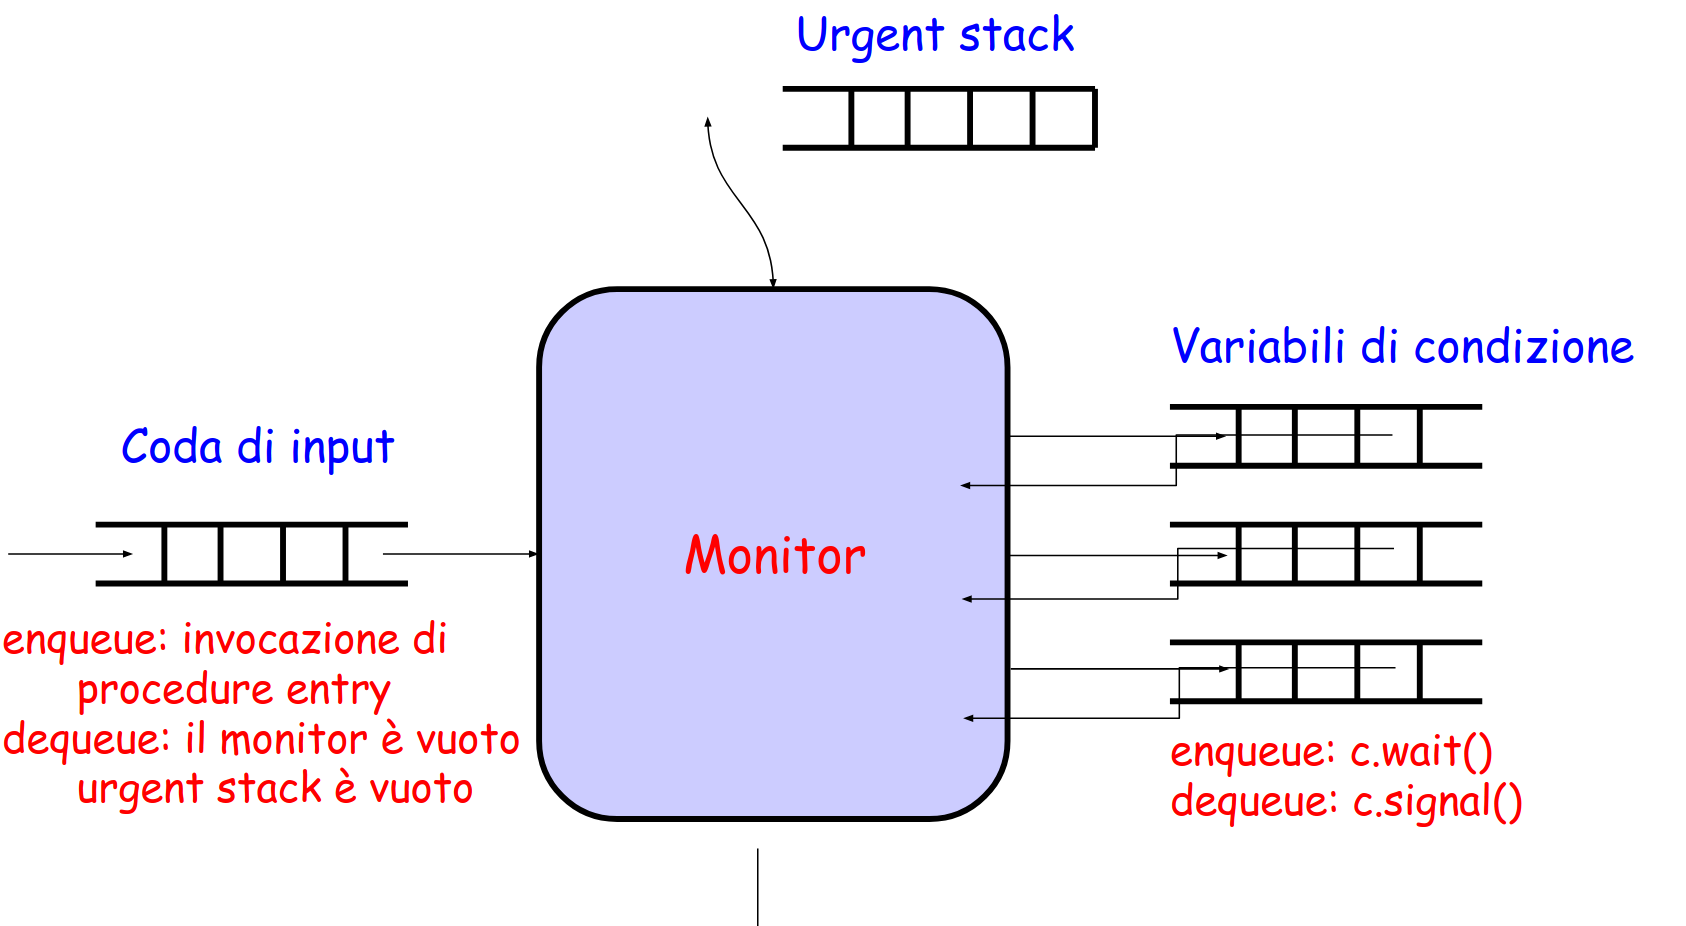
\includegraphics[width=0.7\linewidth]{Images/Screenshot 2025-01-16 at 12-18-56 so-03.1-concorrenza - so-03.1-concorrenza.pdf.png}
\end{figure}

\subsubsection{ wait/signal vs P/V}

A prima vista \textbf{wait e signal} potrebbero sembrare simili alle operazioni sui semafori \textbf{P e V}, ma in verità ci sono differenze sostanziali.

\begin{itemize}
    \item \textbf{signal} non ha alcun effetto se nessun processo sta attendendo la condizione. Mentre \textbf{V} "memorizza" il verificarsi degli eventi.
    \item \textbf{wait} è sempre bloccante, \textbf{P} (se il semaforo ha valore positivo) no.
    \item Il processo risvegliato dalla \textbf{signal} viene eseguito per primo.
\end{itemize}

\subsubsection{Politiche di signaling}
Signal urgent è la politica "classica" di signaling.
SU - signal urgent.

Ne esistono altre..

\subsection{Implementazione dei semafori}

\begin{lstlisting}
monitor Semaphore {
    int value;
    condition c; /* value > 0 */

    procedure entry void P() {
        value--;
        if (value < 0)
            c.wait();
    }

    procedure entry void V() {
        value++;
        c.signal();
    }

    Semaphore(int init) {
        value = init;
    }
}
\end{lstlisting}
\newpage

\subsection{Monitor - R/W}
\begin{lstlisting}
process Reader {
    while (true) {
        rwController.startRead();
        //read the database
        rwController.endRead();
    }
}

process Writer {
    while (true) {
        rwController.startWrite();
        //write the database
        rwController.endWrite();
    }
}
\end{lstlisting}
\newpage
\begin{lstlisting}
monitor RWController
    int nr; /* number of readers */
    int nw; /* number of writers */
    condition okToRead; /* nw == 0 */
    condition okToWrite; /* nr == 0 && nw == 0 */

    procedure entry void startRead() {
        if (nw != 0)
            okToRead.wait();
            nr = nr + 1;

        if (nw == 0) /* always true */
            okToRead.signal();
        
        if (nw == 0 && nr == 0) /* always false */
            okToWrite.signal();
}

    procedure entry void endRead() {
        nr = nr - 1;
        if (nw == 0) /* true but useless */
            okToRead.signal();

        if (nw == 0 && nr == 0)
            okToWrite.signal();
    }

    procedure entry void startWrite() {
        if (!(nr==0 && nw==0))
            okToWrite.wait();
            nw = nw + 1;

        if (nw == 0) /* always true */
            okToRead.signal();

        if (nw == 0 && nr == 0) /* always false */
            okToWrite.signal();
}

    procedure entry void endWrite() {
        nw = nw - 1;
        if (nw == 0) /* Always true */
            okToRead.signal();
        
        if (nw == 0 && nr == 0)
            okToWrite.signal();
        }

    RWController() { /* Constructor */
        nr = nw = 0;
    }

\end{lstlisting}

E' possibile semplificare il codice eliminando le righe if quando sempre vere, eliminando le righe if e il ramo opportuno quando sempre falso.
\newpage
\subsubsection{Monitor - R/W semplificato}
\begin{lstlisting}
    procedure entry void startRead() {
        if (nw != 0) okToRead.wait();
            nr = nr + 1;
            okToRead.signal();
    }

    procedure entry void endRead() {
        nr = nr - 1;
        if (nr == 0) 
            okToWrite.signal();
    }

    procedure entry void startWrite() {
        if (!(nr=0 && nw =0)) 
            okToWrite.wait();
            nw = nw + 1;
    }

    procedure entry void endWrite() {
        nw = nw - 1;
        okToRead.signal();
        if (nw == 0 && nr == 0) 
            okToWrite.signal();
    }
\end{lstlisting}

\subsection{Monitor - Produttore / consumatore}
\begin{lstlisting}
process Producer {
    Object x;
    while (true) {
        x = produce();
        pcController.write(x);
    }
}

process Consumer {
    Object x;
    while (true) {
        x = pcController.read();
        consume(x);
    }
}
\end{lstlisting}
\newpage
\begin{lstlisting}
monitor PCController {
    Object buffer;
    condition empty;
    condition full;
    boolean isFull;

    PCController() {
        isFull=false;
    }


    procedure entry Object read() {
        if (!isFull)
            full.wait();
    
        int retvalue = buffer;
        isFull = false;
        empty.signal();
        return retvalue;
    }

    procedure entry void write(int val) {
        if (isFull)
            empty.wait();
   
        buffer = val;
        isFull = true;
        full.signal();
        }
    }
\end{lstlisting}

\subsection{Monitor - Buffer limitato }
\begin{lstlisting}
monitor PCController {
    Object[] buffer;
    condition okRead, okWrite;
    int count, rear, front;

    PCController(int size) {
        buffer = new Object[size];
        count = rear = front = 0;
    }

    procedure entry Object read() {
        if (count == 0)
            okRead.wait();

        int retval = buffer[rear];
        cont--;
        rear = (rear+1) % buffer.length;
        okWrite.signal();
        return retval;
    }
    
    procedure entry void write(int val) {
        if (count == buffer.length)
            okWrite.wait();
        buffer[front] = val;
        count++;
        front = (front+1) %
        buffer.length;
        okRead.signal();
    }
\end{lstlisting}

\subsection{Monitor - Filosofi a cena (no deadlock)}
\begin{lstlisting}
    process Philo[i] {
        while (true) {
            //think
            chopstick[MIN(i,i+1)].pickup();
            chopstick[MAX(i,i+1)].pickup();
            //eat
            chopstick[MIN(i,i+1)].putdown();
            chopstick[MAX(i,i+1)].putdown();
        }
    }
\end{lstlisting}

\begin{lstlisting}
    monitor DPController {
        condition[] unusedchopstick = new condition[5];
        boolean[] chopstick = new boolean[5];
      
        procedure entry void startEating(int i) {
        
        if (chopstick[i])
            unusedchopstick[i].wait();
            chopstick[i] = true;

        if (chopstick[i+1])
            unusedchopstick[i+1].wait();
            chopstick[i+1] = true;
        }

        procedure entry void finishEating(int i) {
            chopstick[i] = false;
            chopstick[i+1] = false;
            unusedchopstick[i].signal();
            unusedchopstick[i+1].signal();
        }
    }

monitor chopstick[i] {
    boolean inuse = false;
    condition free;
   
    procedure entry void pickup() {
        if (inuse)
            free.wait();
            inuse = true;
    }

    procedure entry void putdown() {
        inuse = false;
        free.signal();
    }
   
\end{lstlisting}    

\newpage

\subsection{Implementazione dei monitor tramite semafori}
\paragraph{Ingredienti:}
\begin{itemize}
    \item un modulo di gestione stack (per urgent)
    \begin{lstlisting}
        interface Stack {
            void push(Object x);
            Object pop();
            boolean empty();
        }
    \end{lstlisting}

    \item un semaforo di mutua esclusione \textbf{e}
    \item per ogni variabile di condizione $cond_i$, una coppia ($c_i$, $nc_i$).
    $c_i$ è un semaforo correlato alla condizione, inizializzato a 0. $nc_i$ è il numero di processi che sono in attesa del verificarsi della condizione.
    \item un "allocatore" di semafori \textit{(o alternativamente un semaforo per ogni processo)}.
\end{itemize}

\begin{lstlisting}
    //Inizializzazione
        Semaphore e = new Semaphore(1);
        Stack stack = new Stack();

    //Entrata nel monitor
        e.P();
    
    //Wait su cond_i
        nc_i++;
        if (!stack.empty()) {
            Semaphore s = stack.pop();
            s.V();
        } else {
            e.V();
        }
        c_i.P();

    //Signal su cond_i
        if (nci > 0) {
            nc_i--;
            ci.V();
            Semaphore s = new Semaphore(0);
            stack.push(s);
            s.P();
            /* free(s) / garbage coll. */
        }

    //Uscita dal monitor
        if (!stack.empty()) {
            Semaphore s = stack.pop();
            s.V();
        } else {
            e.V();
    }
\end{lstlisting}

\newpage
\section{Message passing}
\subsection{Introduzione}
Abbiamo già visto paradigmi di sincronizzazione come: semafori, monitor. In questi paradigmi, la comunicazione avviene tramite memoria condivisa.

I paradigmi di comunicazione come il \textbf{message passing} permettono la comunicazione tra processi tramite messaggi.

La sincronizzazione avviene tramite lo scambio di messaggi, e non più semplici segnali.

\subsubsection{Definizioni}
Un \textbf{messaggio} è un insieme di informazioni formattate da un processo mittente e interpretate da un processo destinatario.

Un meccanismo di "\textbf{scambio di messaggi}" copia le informazioni di un messaggio da uno spazio di indirizzamento
di un processo allo spazio di indirizzamento di un altro processo.
\begin{figure} [h]
    \centering
    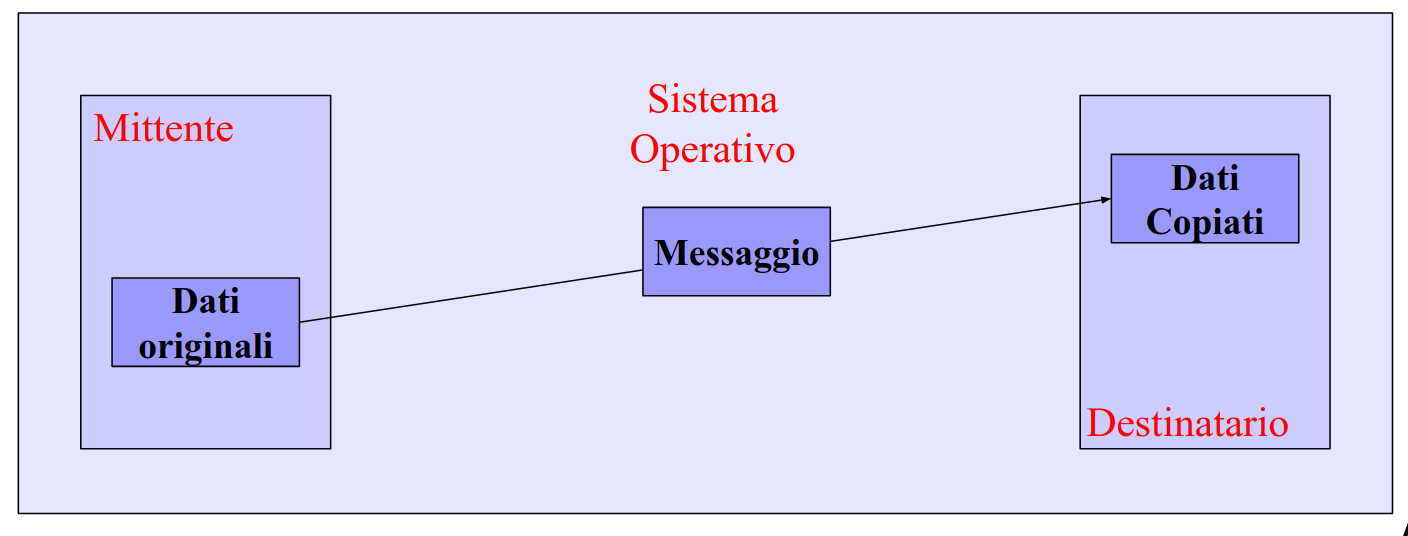
\includegraphics[width=0.7\linewidth]{Images/Screenshot 2025-01-16 at 13-01-13 so-03.1-concorrenza - so-03.1-concorrenza.pdf.png}
\end{figure}

\subsubsection{Operazioni}
\paragraph{send:} utilizzata dal processo mittente per "spedire" un messaggio ad un processo destinatario specificato.
\paragraph{receive:} utilizzata dal processo destinatario per "ricevere" un messaggio da un processo mittente. Il processo mittente può essere specificato, o no.

Il passaggio dallo spazio di indirizzamento del mittente a quello del destinatario è mediato dal sistema operativo (protezione memoria), il processo destinatario deve eseguire un'operazione receive per ricevere qualcosa.

\subsubsection{Tassonomia}
\begin{itemize}
    \item MP sincrono \begin{itemize}
        \item Send sincrono
        \item Receive bloccante
    \end{itemize}
    \item MP asincrono \begin{itemize}
        \item Send asincrono
        \item Receive bloccante
        \end{itemize}
    \item MP completamente asincrono \begin{itemize}
        \item Send asincrono
        \item Receive non bloccante
        \end{itemize}
\end{itemize}

\subsection{MP sincrono}
\subsubsection{Operazione send sincrona}
Sintassi: \lstinline{ssend(m, q)}.

Il mittente p spedisce il messaggio m al processo q, restando bloccato fino a quando q non esegue l'operazione \lstinline{sreceive(m, p)}.

\subsubsection{Operazione receive bloccante}
Sintassi: \lstinline{m = sreceive(p)}

Il destinatario q riceve il messaggio m dal processo p; se il mittente non ha ancora spedito alcun messaggio, il destinatario si blocca in attesa di ricevere un messaggio, è possibile lasciare il mittente non specificato (utilizzando *).


\subsection{MP asincrono}
\subsubsection{Operazione send asincrona}
Sintassi: \lstinline{asend(m, q)}.

il mittente p spedisce il messaggio m al processo q, senza bloccarsi in attesa che il destinatario esegua l'operazione \lstinline{areceive(m, p)}.

\subsubsection{Operazione receive bloccante}
Sintassi: \lstinline{m = areceive(p)}

Il destinatario q riceve il messaggio m dal processo p; se il mittente non ha ancora spedito alcun messaggio, il destinatario si blocca in attesa di ricevere un messaggio, è possibile lasciare il mittente non specificato (utilizzando *).

\subsection{MP completamente asincrono}
\subsubsection{Operazione send asincrona}
Sintassi: \lstinline{asend(m, q)}.

il mittente p spedisce il messaggio m al processo q, senza bloccarsi in attesa che il destinatario esegua l'operazione \lstinline{nb-receive(m, p)}.

\subsubsection{Operazione receive non bloccante}
Sintassi: \lstinline{m = nb-receive(p)}

Il destinatario q riceve il messaggio m dal processo p; se il mittente non ha ancora spedito alcun messaggio, la nb-receive termina ritornando un messaggio "nullo", è possibile lasciare il mittente non specificato (utilizzando *).

\begin{figure} [h]
    \centering
    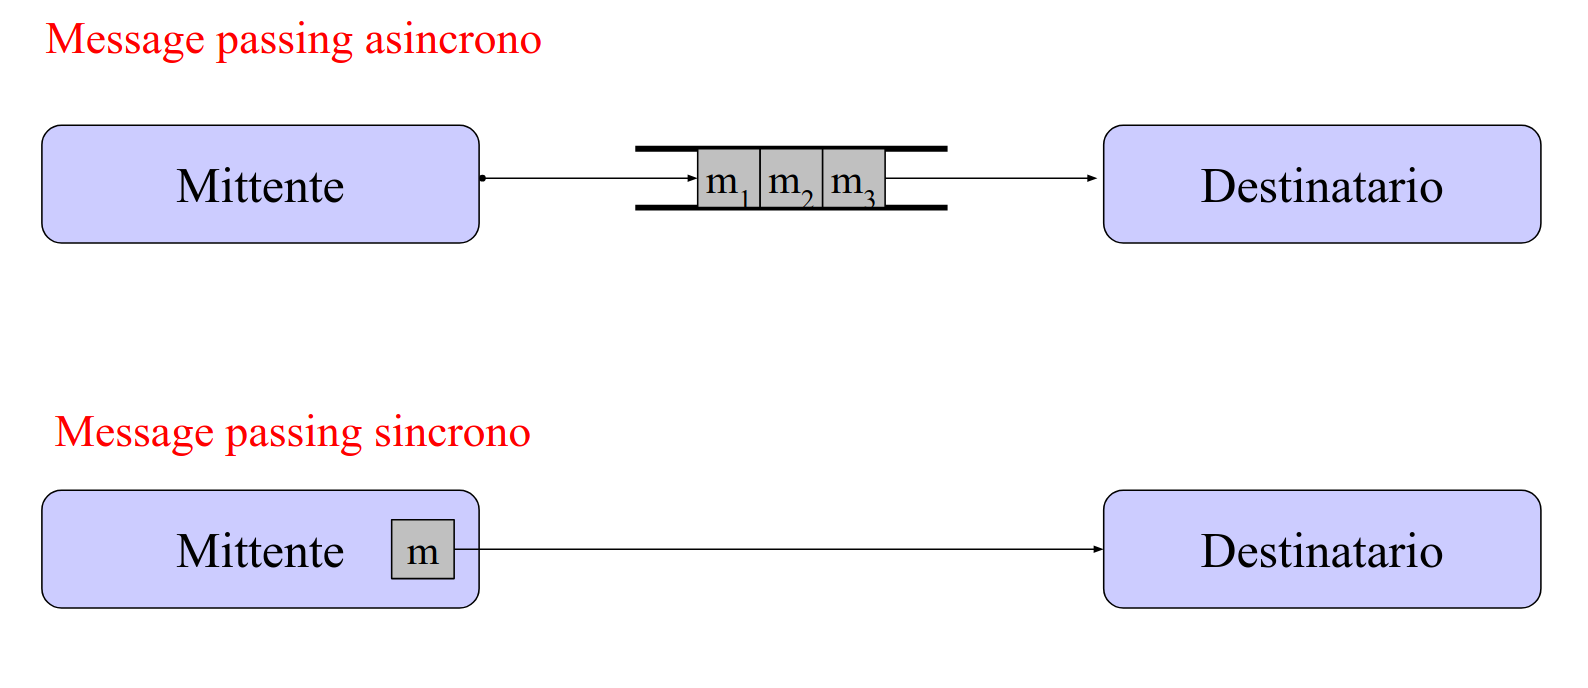
\includegraphics[width=0.7\linewidth]{Images/Screenshot 2025-01-16 at 13-17-46 so-03.1-concorrenza - so-03.1-concorrenza.pdf.png}
\end{figure}

In letteratura ci sono numerose diverse sintassi per descrivere message passing.
Ad esempio, invece che indicare il processo destinazione/mittente, si indica il nome di un canale.

Message passing asincrono con 3 primitive principali: send, receive, reply (Thoth). Non la receive, ma solamente la reply sblocca il mittente, utile per rendere MP simile alle chiamate di procedura remota.
\newpage
\subsection{MP sincrono dato quello asincrono}
\begin{lstlisting}
void ssend(Object msg, Process q) {
    asend(msg, q);
    ack = areceive(q);
}

Object sreceive(p) {
    Object msg = areceive(p);
    asend(ack, p);
    return msg;
}
\end{lstlisting}

\begin{lstlisting}
/* p identifies the calling process */

void asend(Object m, Process q) {
    ssend(SND(m,p,q), server);
}

void areceive(Process q) {
    ssend(RCV(p,q), server);
    Object m = sreceive(server);
    return m;
}

process server {
/* One element x process pair */
    int[][] waiting;
    Queue[][] queue;
    while (true) {
        handleMessage();
    }
}

void handleMessage() {
    msg = sreceive(*);
    if (msg == <SND(m,p,q)>) {
        if (waiting[p,q]>0) {
            ssend(m, p);
            waiting[p,q]--;
        } else {
            queue[p,q].add(m);
        }
    }   else if (msg == <RCV(q,p)>) {
            if (queue[p,q].isEmpty()) {
                waiting[p,q]++;
            } else {
                m = queue[p,q].remove();
                ssend(m, dest);
            }
        }
    }
\end{lstlisting}
\newpage
\subsection{Message Passing - Filosofi a cena}
\begin{lstlisting}
process Philo[i] {
    while (true) {
    //think
    asend(<PICKUP,i>, chopstick[MIN(i, (i+1)%5)]);
    msg = areceive(chopstick[MIN(i, (i+1)%5)]);
    asend(<PICKUP,i>, chopstick[MAX(i, (i+1)%5)]);
    msg = areceive(chopstick[MAX(i, (i+1)%5)]);
    //eat
    asend(<PUTDOWN,i>, chopstick[MIN(i, (i+1)%5)]);
    asend(<PUTDOWN,i>, chopstick[MAX(i, (i+1)%5)]);
    }
}
\end{lstlisting}

\begin{lstlisting}
process chopstick[i] {
    boolean free = true;
    Queue queue = new Queue();
    while (true) {
        handleRequests();
    }
}

void handleRequests() {
    msg = areceive(*);
    if (msg == <PICKUP,j>) {
        if (free) {
            free = false;
            asend(ACK, philo[j]);
        } else {
            queue.add(j);
        }
    } else
        if (msg == <PUTDOWN, j>) {
            if (queue.isEmpty()) {
                free = true;
            } else {
                k = queue.remove();
                asend(ACK, philo[k]);
            }
        }
}
\end{lstlisting}
\newpage
\subsection{Message Passing - Produttori e consumatori}
\begin{lstlisting}
process Producer {
    Object x;
    while (true) {
        x = produce();
        ssend(x, PCmanager);
    }
}

process Consumer{
    Object x;
    while (true) {
        x = sreceive(PCmanager);
        consume(x);
    }
}

process PCmanager {
    Object x;
    while (true) {
        x = sreceive(Producer);
        ssend(x, Consumer);
    }
}
\end{lstlisting}

\section{Conclusioni} 
\subsection{Riassunto}
\begin{itemize}
    \item \textbf{Semafori:} fondamentale primitiva di sincronizzazione, effettivamente offerta dai S.O. . Di livello troppo basso; facile commettere errori.
    \item  \textbf{Monitor:} meccanismi integrati nei linguaggi di programmazione, pochi linguaggi di larga diffusione sono dotati di monitor; unica eccezione Java, con qualche distinguo.
    \item \textbf{Message passing:} da un certo punto di vista, il meccanismo più diffuso. Può essere poco efficiente (copia dati tra spazi di indirizzamento).
\end{itemize}
\subsection{Potere espressivo}
\paragraph{Definizione:} Si dice che il paradigma di programmazione A è espressivo almeno quanto il paradigma di programmazione B (e si scrive $A \ge B$) quando è possibile esprimere ogni programma scritto con B mediante A.

Ovvero, quando è possibile scrivere una libreria che consenta di implementare le chiamate di un paradigma B esprimendole in termini di A si avrà $A \ge B$.
\newline
Si dice che due paradigmi hanno lo stesso potere espressivo se $A \ge B$ e $B \ge A$.

In vari punti di questi lucidi si mostrano delle relazioni tra i vari paradigmi di programmazione mediante funzioni di implementazione.

Si possono tracciare le seguenti classi di paradigmi:
\begin{itemize}
    \item \textbf{Metodi a memoria condivisa:}
    \begin{itemize}
        \item semafori, semafori binari, monitor hanno tutti lo stesso potere espressivo.
        \item dekker e peterson, Test\&Set necessitano di busy waiting.
    \end{itemize}
    
    \item \textbf{Metodi a memoria privata:} message passing asincrono (ha maggiore potere espressivo) e message passing sincrono.
\end{itemize}
